\chapter{Introduction}
\label{chap:01}


\paragraph{}


 Models in cell biology are both familiar and mysterious. On the one hand, biologists have traditionally utilised models to represent reality, such as diagrams, rules, graphs, plots, chemical formulas, and relationships. Their purpose is to be similar to numerous organisms while not being the same. As a result, it is reasonable to suppose that discoveries will also shed light on the workings of other organisms. On the other hand, a mathematical representation of biological systems and processes can be understood as a model, forming a relatively recent branch of biological study. A mathematical model, according to Eykhoff \cite{serra2011using}, is "a representation of the main elements of an existing system (or a system to be developed) that offers knowledge of that system in useable form." Mathematical models can take numerous forms and are especially effective for data-integrative studies of interactions between different components of biological systems and the way these interactions affect the overall function and behaviour of a system \cite{kapur1988mathematical}. This processes biological modelling approach connects fundamental chemical and physical principles, prior knowledge of the researched system, and experimental data to create a robust tool for extending and formalising classical cell biology \cite{motta2013mathematical,friedman2014mathematical}. Unscrambling an organism's genome is undoubtedly a first step toward understanding mechanisms in living cells; nevertheless, a complete image is required to truly capture the regulatory features of genetic, metabolic, and cellular signalling networks \cite{gold1977mathematical}. This is supported by mathematical formulation, hypothesis creation, and comparison validation with experimental data \cite{almeida2021formulation}. Data-driven calibrated models have the ability to generate new hypotheses and predictions, and they represent a guided approach to building promising continuous experiments to investigate issues that are not susceptible to experimental investigation. Simultaneously, experiment results are frequently too complicated to be understood by visual examination and can be related.
 


\section{Background of the study}
\label{sec:1.1}

\paragraph{}

The study of linked mathematical modeling has since become an essential branch of mathematics, with applications in physics, biology, and chemistry \cite{fowler1997mathematical}. A simulation is a mathematical depiction of a physical, biological, or information system.  Models enable us to think about a system and forecast its behaviour. A dynamical system is one in which the consequences of actions do not arise instantly.  For example, a headache does not go away immediately after taking aspirin; it takes time to take action. Additional funding for a development project does not enhance profits in the  short term, but it may do the same in the longer - term in enterprise applications. These are dynamic systems instances in which the system's behaviour varies over time. Most species directly correspond to numerous patterns in our environment, such as the earth's rotation around the sun, the alternation of night and day, or the tides. But in this project, mathematical modeling for cancer signalling will be discussed. 


\subsection{Mathematical modeling approaches}
\paragraph{}

There are many different approaches to mathematical modeling that can be used in the study of cancer. The choice of approach will depend on the specific research question being addressed and the characteristics of the cancerous system being studied. Some common approaches to mathematical modeling in cancer research include:

\begin{itemize}
    \item Deterministic models: These models can be used to describe the relationships between different signalling pathways and the behaviour of cancer cells and to predict the effects of different perturbations on the system \cite{altrock2015mathematics}, such as mutations or the inhibition of specific signalling proteins \cite{tabassum2019mathematical}.

    \item Stochastic models: These models can be used to describe the randomness or uncertainty inherent in cancerous systems and can be used to study how random events, such as gene mutations, contribute to the development and progression of cancer \cite{tsodikov1996stochastic}.

    \item Agent-based models: These models can be used to represent the behaviour of individual cancer cells or the interactions between cancer cells and the surrounding tissue and can be used to study how the collective behaviour of cancer cells emerges from their individual behaviour \cite{figueredo2013investigating}.

    \item Network models: These models can be used to represent the interactions between different signalling pathways and molecules in cancerous systems and can be used to study how these interactions contribute to the development and progression of cancer \cite{ji2020mathematical}.

    \item Dynamical systems models: These models can be used to describe the evolution of cancerous systems over time and can be used to study how cancer cells adapt and respond to different stimuli or perturbations \cite{haupt2021mathematical}.
\end{itemize}

Again, these are just a few examples, and researchers may use a combination of different approaches to best capture the behaviour of a particular cancerous system. All strategies include assumptions about the system under consideration, necessitate specific sorts of measurements, and allow for conclusions with varying degrees of accuracy and detail.





%  \begin{figure}[hbt!]
% 	\centering
% 	\begin{framed}
% 	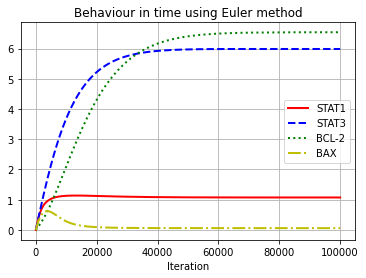
\includegraphics[width=0.6\textwidth]{Figures/A.JPG}
% 	\end{framed}
% 	\caption{Two blocks are attached to three springs \cite{Departme83:online}.}
% 	\label{fig:1}
% \end{figure}


\subsection{Mathematical modelling for cell signalling}

The term "biological system" can be interpreted in a variety of ways at different organisational levels, necessitating unique approaches and methodologies for modelling and analysis. Metabolic systems, cell cycle regulation, development and differentiation, as well as intra- and intercellular signalling and cell communication, are all included. The majority of the related underlying processes exhibit dynamic activity. Changes in gene expression patterns or metabolite profiles, as well as fluctuations in protein and hormone levels, are examples of this, particularly in response to altered environmental conditions or pharmacological modulation \cite{feitelson2015sustained}. Cellular signalling is a component of complex system communication, directing basic as well as cell-type specific cellular functions and coordinating cell actions in unicellular and multicellular organisms \cite{danos2007rule}. Beginning with the activation of a cell surface receptor, intracellular signalling molecules are then changed, allowing the evoked initial signal to be transmitted to the targeted cell response. These signalling events do not always go in a straight line, relaying and regulating information from cell surface receptors to effectors like transcription factors or specific enzymes. Cellular signalling networks are made up of highly coupled modules that regulate many processes in context, including regulatory feedback \cite{jordan2000interleukin}.

\section{Problem statement and objectives}
\paragraph{}

Apoptosis is a crucial biological process that regulates cell death in response to various stimuli. It is a complex process that involves several key signaling pathways and intercellular modules. The Intercellular modules such as STAT1, STAT3, Bcl-2 and BAX play a critical role in apoptosis signaling. Understanding the dynamics of these modules and how they interact with each other is crucial for gaining insights into the apoptosis process.

This project aims to conduct numerical investigations of the Intercellular modules (STAT1, STAT3, Bcl-2, and BAX) involved in apoptosis signalling. The project will focus on two methods for numerical investigations, namely Euler's method and the Runge-Kutta fourth-order method. The main focus of this project is to understand the behavior of these modules in response to the activation of the IFN-$\beta$ and JAK2 signalling pathways.

Euler's method is a basic numerical method used to solve ordinary differential equations (ODEs). It is a simple method that uses a straight-line approximation to estimate the solution to an ODE. However, Euler's method is not very accurate and can be prone to error, especially when the solution changes rapidly. Despite this, it is still widely used as a first step in solving ODEs, as it provides a simple and straightforward approach to solving ODEs.

The Runge-Kutta fourth-order method is a more sophisticated numerical method that provides improved accuracy compared to Euler's method. It uses a combination of multiple straight-line approximations to estimate the solution to an ODE. This method is considered more accurate and efficient compared to Euler's method and is commonly used to solve complex ODEs.

The numerical investigations will be conducted by representing the levels of the Intercellular modules (STAT1, STAT3, Bcl-2, and BAX) and their activity by mathematical variables. The behaviour of the modules will be analyzed and compared using both Euler's method and the Runge-Kutta fourth-order method. The results of the numerical investigations will be visualized and compared, allowing for a better understanding of the behaviour of the Intercellular modules in response to the activation of the IFN-$\beta$ and JAK2 signalling pathways.

The mathematical equilibrium and stability analysis will involve finding the steady-state solutions and determining their stability for the systems representing the Intercellular modules and their interactions. The equilibrium and stability analysis results will provide essential insights into the long-term behaviour of the modules.

In conclusion, this project aims to provide a deeper understanding of the behaviour of Intercellular modules (STAT1, STAT3, Bcl-2, and BAX) involved in apoptosis signalling by combining the mathematical equilibrium and stability analysis and numerical investigations. The numerical investigations using Euler's method and the Runge-Kutta fourth-order method will provide valuable insights into the dynamics of these modules and their interactions with each other. This project is expected to contribute to the field of apoptosis research and provide a foundation for further studies on the apoptosis signalling network.



\section{Project structure}
\paragraph{}

This project focuses on mathematical modeling approaches for cell signalling and aims to understand the genetic alterations in signalling pathways in cancer and their downstream signalling. The project starts with a background of the study where mathematical modelling approaches and their application for cell signalling are introduced. The problem statement and objectives are then highlighted. The project structure is outlined, which includes the theoretical background, methodology, numerical method for ordinary differential equations, results and discussion, and conclusion.

The theoretical background covers a biological introduction of cell signalling and explains genetic alterations in signalling pathways and their relevance to cancer. It provides an in-depth look at receptor tyrosine kinases in cancer and their downstream signalling, along with a summary of the current state of knowledge about the signalling pathways involved in cancer and the challenges in understanding these pathways. Numerical analysis is also briefly mentioned.

The methodology section of the project explains the biological approach of STAT1, STAT3, Bcl-2 and BAX and then moves on to a mathematical model for the intracellular module of these proteins. The mathematical model includes a schematic diagram of the apoptosis signalling network and the governing ordinary differential equations for the intracellular signalling network. The section concludes with mathematical equilibrium and stability analysis.

The numerical method for ordinary differential equations section explains the numerical investigation using Euler’s method, the numerical integration technique for the Runge-Kutta fourth-order method, and other relevant details. The results and discussion section present the numerical results for different scenarios, such as S=0 and J=0, S=0 and J=1, S=0.4 and J=0, and S=1 and J=1. The section concludes with an equilibrium and stability analysis.

The project concludes with a summary of the findings and recommendations for future research.  
\paragraph{}






































